\chapter{Linux Internals}

\section{Introduction}

Linux is one of the most widely used operating systems in the world. It powers servers, cloud infrastructure, embedded devices, supercomputers, smartphones (via Android), and modern backend systems.

For Software Development Engineer (SDE) interviews, Linux internals form a critical topic because they connect operating system theory with real-world system implementation.

\section{Linux Architecture Overview}

Linux follows a layered architecture.

\begin{figure}[H]
\centering
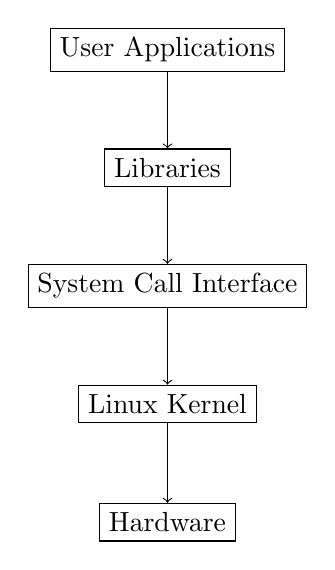
\begin{tikzpicture}
\node[draw] (apps) at (0,6) {User Applications};
\node[draw] (libs) at (0,4.5) {Libraries};
\node[draw] (syscalls) at (0,3) {System Call Interface};
\node[draw] (kernel) at (0,1.5) {Linux Kernel};
\node[draw] (hardware) at (0,0) {Hardware};

\draw[->] (apps)--(libs);
\draw[->] (libs)--(syscalls);
\draw[->] (syscalls)--(kernel);
\draw[->] (kernel)--(hardware);
\end{tikzpicture}
\caption{Linux Architecture}
\end{figure}

Major components include:

\begin{itemize}
\item User Space
\item System Call Interface
\item Kernel Space
\item Hardware Layer
\end{itemize}

\section{User Space vs Kernel Space}

Linux divides execution into two protection domains.

\subsection{User Space}

Applications execute in user mode.

Characteristics:

\begin{itemize}
\item Restricted privileges
\item Cannot access hardware directly
\item Cannot execute privileged instructions
\end{itemize}

\subsection{Kernel Space}

Kernel executes in privileged mode.

Characteristics:

\begin{itemize}
\item Full hardware access
\item Memory management
\item Scheduling
\item Device management
\end{itemize}

\begin{table}[H]
\centering
\begin{tabular}{lll}
\toprule
Feature & User Space & Kernel Space \\
\midrule
Privilege & Low & High \\
Hardware Access & No & Yes \\
Memory Access & Restricted & Full \\
Crash Impact & Process Only & Entire System \\
\bottomrule
\end{tabular}
\caption{User Space vs Kernel Space}
\end{table}

\section{Linux Kernel Architecture}

The Linux kernel contains several subsystems.

\begin{figure}[H]
\centering
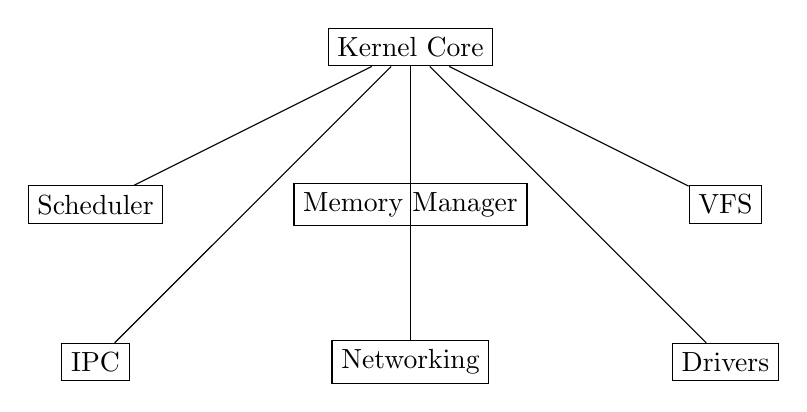
\begin{tikzpicture}
\node[draw] (sched) at (-4,0) {Scheduler};
\node[draw] (mm) at (0,0) {Memory Manager};
\node[draw] (vfs) at (4,0) {VFS};

\node[draw] (ipc) at (-4,-2) {IPC};
\node[draw] (net) at (0,-2) {Networking};
\node[draw] (drv) at (4,-2) {Drivers};

\node[draw] (core) at (0,2) {Kernel Core};

\draw (core)--(sched);
\draw (core)--(mm);
\draw (core)--(vfs);
\draw (core)--(ipc);
\draw (core)--(net);
\draw (core)--(drv);
\end{tikzpicture}
\caption{Linux Kernel Subsystems}
\end{figure}

\section{Monolithic Kernel Design}

Linux uses a monolithic kernel.

Characteristics:

\begin{itemize}
\item All major services run in kernel space
\item High performance
\item Shared address space
\end{itemize}

Advantages:

\begin{itemize}
\item Fast communication
\item Lower overhead
\item Better performance
\end{itemize}

Disadvantages:

\begin{itemize}
\item Large codebase
\item Bug may crash entire system
\end{itemize}

\section{Kernel Modules}

Kernel modules are dynamically loadable components.

Examples:

\begin{itemize}
\item Device drivers
\item File systems
\item Network protocols
\end{itemize}

Common commands:

\begin{lstlisting}[style=interviewcode,basicstyle=\ttfamily\small]
lsmod
insmod module.ko
rmmod module
modprobe module
\end{lstlisting}

Benefits:

\begin{itemize}
\item Extensibility
\item Reduced kernel size
\item Runtime loading
\end{itemize}

\section{System Call Interface}

System calls provide controlled access to kernel services.

Examples:

\begin{itemize}
\item open()
\item read()
\item write()
\item fork()
\item execve()
\item mmap()
\end{itemize}

\begin{figure}[H]
\centering
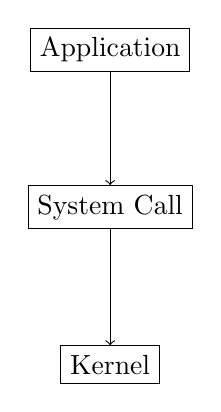
\begin{tikzpicture}
\node[draw] (app) at (0,4) {Application};
\node[draw] (sys) at (0,2) {System Call};
\node[draw] (kernel) at (0,0) {Kernel};

\draw[->] (app)--(sys);
\draw[->] (sys)--(kernel);
\end{tikzpicture}
\caption{System Call Flow}
\end{figure}

\section{Process Management in Linux}

Linux represents processes using the \texttt{task\_struct} structure.

Information stored:

\begin{itemize}
\item PID
\item State
\item Memory mappings
\item Open files
\item Scheduling information
\end{itemize}

Common process states:

\begin{itemize}
\item Running
\item Ready
\item Sleeping
\item Stopped
\item Zombie
\end{itemize}

\section{Scheduler Overview}

The scheduler decides which task gets CPU time.

Goals:

\begin{itemize}
\item Fairness
\item Throughput
\item Low latency
\item Scalability
\end{itemize}

\section{Completely Fair Scheduler (CFS)}

CFS is the default Linux scheduler.

Core idea:

\begin{quote}
Every runnable process should receive a fair share of CPU time.
\end{quote}

CFS maintains a Red-Black Tree ordered by virtual runtime.

\begin{figure}[H]
\centering
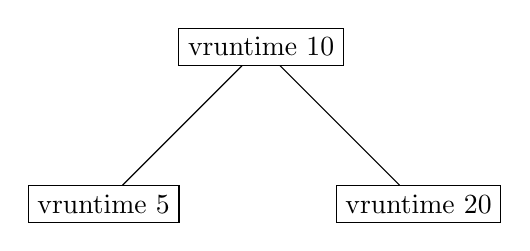
\begin{tikzpicture}
\node[draw] (root) at (0,2) {vruntime 10};
\node[draw] (l) at (-2,0) {vruntime 5};
\node[draw] (r) at (2,0) {vruntime 20};

\draw (root)--(l);
\draw (root)--(r);
\end{tikzpicture}
\caption{Simplified CFS Tree}
\end{figure}

Process with smallest virtual runtime executes next.

\section{Linux Memory Management}

Linux memory management includes:

\begin{itemize}
\item Physical memory management
\item Virtual memory
\item Paging
\item Page cache
\item Slab allocator
\end{itemize}

Memory zones:

\begin{itemize}
\item DMA
\item Normal
\item High Memory
\end{itemize}

\section{Virtual Memory in Linux}

Each process receives a private virtual address space.

Advantages:

\begin{itemize}
\item Isolation
\item Security
\item Larger logical memory
\item Shared libraries
\end{itemize}

Key concepts:

\begin{itemize}
\item Page Tables
\item TLB
\item Demand Paging
\item Swap
\end{itemize}

\section{Linux File Systems Overview}

Linux supports multiple file systems.

Examples:

\begin{itemize}
\item ext4
\item XFS
\item Btrfs
\item NFS
\item tmpfs
\end{itemize}

The Virtual File System (VFS) provides a unified interface.

\section{ext4 Architecture}

ext4 is the most common Linux file system.

Features:

\begin{itemize}
\item Journaling
\item Extents
\item Delayed Allocation
\item Large File Support
\end{itemize}

Disk layout:

\begin{figure}[H]
\centering
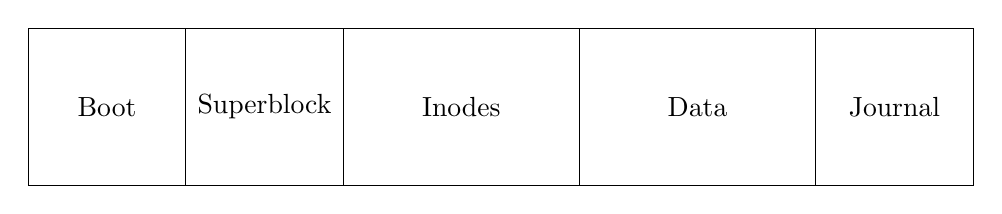
\begin{tikzpicture}
\draw (0,0) rectangle (12,2);

\draw (2,0)--(2,2);
\draw (4,0)--(4,2);
\draw (7,0)--(7,2);
\draw (10,0)--(10,2);

\node at (1,1) {Boot};
\node at (3,1) {Superblock};
\node at (5.5,1) {Inodes};
\node at (8.5,1) {Data};
\node at (11,1) {Journal};
\end{tikzpicture}
\caption{Simplified ext4 Layout}
\end{figure}

\section{proc File System}

\texttt{/proc} is a virtual file system exposing kernel information.

Examples:

\begin{lstlisting}[style=interviewcode]
cat /proc/cpuinfo
cat /proc/meminfo
cat /proc/self/status
\end{lstlisting}

Uses:

\begin{itemize}
\item Monitoring
\item Diagnostics
\item Performance analysis
\end{itemize}

\section{sysfs}

\texttt{/sys} exposes kernel objects and device information.

Examples:

\begin{lstlisting}[style=interviewcode]
ls /sys/class
ls /sys/devices
\end{lstlisting}

Uses:

\begin{itemize}
\item Device inspection
\item Driver interaction
\item Hardware configuration
\end{itemize}

\section{Signals}

Signals provide asynchronous process notifications.

Common signals:

\begin{table}[H]
\centering
\begin{tabular}{ll}
\toprule
Signal & Purpose \\
\midrule
SIGINT & Interrupt \\
SIGTERM & Graceful Termination \\
SIGKILL & Forced Termination \\
SIGSEGV & Segmentation Fault \\
SIGSTOP & Pause Process \\
\bottomrule
\end{tabular}
\caption{Common Linux Signals}
\end{table}

\section{IPC Mechanisms}

Inter-Process Communication methods include:

\begin{itemize}
\item Pipes
\item Named Pipes
\item Shared Memory
\item Message Queues
\item Semaphores
\item Sockets
\end{itemize}

\section{Daemons}

Daemons are background processes.

Examples:

\begin{itemize}
\item sshd
\item cron
\item systemd
\item nginx
\end{itemize}

Characteristics:

\begin{itemize}
\item No controlling terminal
\item Long-running
\item Service oriented
\end{itemize}

\section{Linux Boot Process}

Linux startup sequence:

\begin{enumerate}
\item Power On
\item BIOS/UEFI
\item Bootloader
\item Kernel Loading
\item Init/Systemd
\item User Services
\end{enumerate}

\begin{figure}[H]
\centering
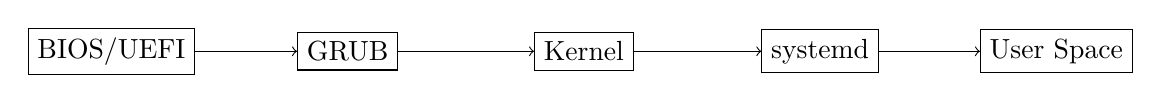
\begin{tikzpicture}
\node[draw] (bios) at (0,0) {BIOS/UEFI};
\node[draw] (boot) at (3,0) {GRUB};
\node[draw] (kernel) at (6,0) {Kernel};
\node[draw] (systemd) at (9,0) {systemd};
\node[draw] (user) at (12,0) {User Space};

\draw[->] (bios)--(boot);
\draw[->] (boot)--(kernel);
\draw[->] (kernel)--(systemd);
\draw[->] (systemd)--(user);
\end{tikzpicture}
\caption{Linux Boot Sequence}
\end{figure}

\section{init and systemd}

Historically Linux used \texttt{init}.

Modern distributions use \texttt{systemd}.

Features:

\begin{itemize}
\item Parallel startup
\item Service management
\item Logging
\item Dependency tracking
\end{itemize}

Commands:

\begin{lstlisting}[style=interviewcode]
systemctl status nginx
systemctl start nginx
systemctl stop nginx
\end{lstlisting}

\section{Kernel Panic}

Kernel panic occurs when the kernel encounters an unrecoverable error.

Causes:

\begin{itemize}
\item Invalid memory access
\item Driver bugs
\item Hardware failures
\item Corrupted kernel structures
\end{itemize}

Result:

\begin{itemize}
\item System halt
\item Diagnostic information displayed
\end{itemize}

\section{Common Linux Commands for OS Interviews}

\begin{table}[H]
\centering
\begin{tabular}{ll}
\toprule
Command & Purpose \\
\midrule
ps & Process Information \\
top & System Monitoring \\
htop & Interactive Monitoring \\
free & Memory Usage \\
vmstat & Virtual Memory Statistics \\
iostat & I/O Statistics \\
lsof & Open Files \\
netstat & Network Statistics \\
ss & Socket Information \\
kill & Send Signal \\
strace & Trace System Calls \\
df & Disk Usage \\
du & Directory Usage \\
\bottomrule
\end{tabular}
\caption{Important Linux Commands}
\end{table}

\section{Real-World Backend Engineering Examples}

\subsection{Web Server}

A high-performance web server:

\begin{itemize}
\item Uses epoll
\item Uses non-blocking sockets
\item Uses multiple worker processes
\end{itemize}

\subsection{Database Server}

A database system:

\begin{itemize}
\item Uses mmap
\item Uses page cache
\item Relies on virtual memory
\end{itemize}

\subsection{Container Platform}

Containers rely on:

\begin{itemize}
\item Namespaces
\item cgroups
\item Process isolation
\end{itemize}

\section{Dedicated Interview Section: What Happens When a Linux Process Starts?}

Process startup sequence:

\begin{enumerate}
\item Parent invokes fork()
\item Child created
\item execve() loads executable
\item Page tables created
\item Program image loaded
\item Dynamic linker resolves libraries
\item main() executes
\end{enumerate}

\begin{figure}[H]
\centering
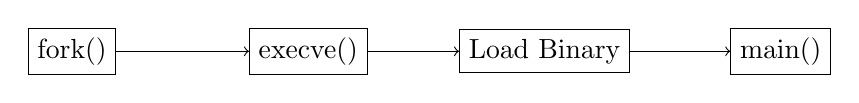
\begin{tikzpicture}
\node[draw] (fork) at (0,0) {fork()};
\node[draw] (exec) at (3,0) {execve()};
\node[draw] (load) at (6,0) {Load Binary};
\node[draw] (main) at (9,0) {main()};

\draw[->] (fork)--(exec);
\draw[->] (exec)--(load);
\draw[->] (load)--(main);
\end{tikzpicture}
\caption{Process Startup}
\end{figure}

\section{Dedicated Interview Section: What Happens When a Process Terminates?}

Termination sequence:

\begin{enumerate}
\item exit() called
\item Resources released
\item Open files closed
\item Exit status stored
\item Process becomes zombie
\item Parent collects status using wait()
\end{enumerate}

\section{Dedicated Interview Section: How a System Call Reaches the Kernel?}

Sequence:

\begin{enumerate}
\item Application invokes library wrapper
\item CPU executes syscall instruction
\item Mode switch occurs
\item Kernel handler executes
\item Service completed
\item Return to user mode
\end{enumerate}

\begin{figure}[H]
\centering
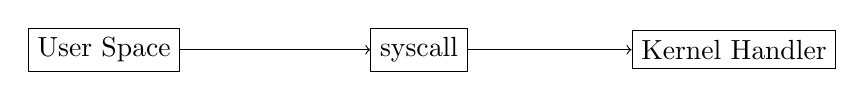
\begin{tikzpicture}
\node[draw] (user) at (0,0) {User Space};
\node[draw] (syscall) at (4,0) {syscall};
\node[draw] (kernel) at (8,0) {Kernel Handler};

\draw[->] (user)--(syscall);
\draw[->] (syscall)--(kernel);
\end{tikzpicture}
\caption{System Call Path}
\end{figure}

\section{Key Takeaways}

\begin{keytakeaways}
Linux is a monolithic kernel operating system that separates execution into user space and kernel space. Processes interact with kernel services through system calls. Process scheduling is handled primarily by the Completely Fair Scheduler (CFS). Linux uses virtual memory, demand paging, and advanced memory allocators for efficiency. ext4 is the most common Linux file system. The proc and sysfs virtual file systems expose kernel and hardware information. Understanding process creation, termination, boot sequence, system calls, and Linux commands is essential for SDE interviews.
\end{keytakeaways}

\section{Interview Questions with Answers}

\begin{enumerate}
\item What is Linux?\\
An open-source Unix-like operating system.

\item What is the Linux kernel?\\
The core component managing hardware and system resources.

\item What is a monolithic kernel?\\
A kernel where major OS services run in kernel space.

\item Difference between user mode and kernel mode?\\
Kernel mode has full privileges; user mode is restricted.

\item What is a system call?\\
An interface to request kernel services.

\item What does fork() do?\\
Creates a new process.

\item What does execve() do?\\
Loads and executes a new program.

\item What is task\_struct?\\
Linux process descriptor structure.

\item What is CFS?\\
Completely Fair Scheduler.

\item What data structure does CFS use?\\
Red-Black Tree.

\item What is virtual memory?\\
An abstraction providing isolated address spaces.

\item What is ext4?\\
A journaling Linux file system.

\item What is VFS?\\
Virtual File System abstraction layer.

\item What is /proc?\\
Virtual filesystem exposing kernel information.

\item What is sysfs?\\
Filesystem exposing kernel objects and devices.

\item What is a signal?\\
An asynchronous notification mechanism.

\item What is SIGKILL?\\
A non-catchable process termination signal.

\item What is IPC?\\
Inter-Process Communication.

\item Name IPC mechanisms.\\
Pipes, shared memory, sockets, message queues.

\item What is a daemon?\\
A background service process.

\item What starts after kernel initialization?\\
systemd or init.

\item What is GRUB?\\
A Linux bootloader.

\item What is a kernel panic?\\
An unrecoverable kernel failure.

\item What happens after exit()?\\
Process becomes zombie until reaped.

\item What command traces system calls?\\
strace.
\end{enumerate}

\section{MCQs with Answers}

\begin{enumerate}

\item Linux primarily uses:
\begin{enumerate}[label=(\alph*)]
\item Microkernel
\item Monolithic Kernel
\item Exokernel
\item Hybrid Kernel
\end{enumerate}
Answer: (b)

\item User applications execute in:
\begin{enumerate}[label=(\alph*)]
\item Kernel Space
\item User Space
\item BIOS
\item Firmware
\end{enumerate}
Answer: (b)

\item System calls transition from:
\begin{enumerate}[label=(\alph*)]
\item Kernel to BIOS
\item User to Kernel
\item Driver to CPU
\item Cache to RAM
\end{enumerate}
Answer: (b)

\item Linux default scheduler is:
\begin{enumerate}[label=(\alph*)]
\item FCFS
\item Round Robin
\item CFS
\item SJF
\end{enumerate}
Answer: (c)

\item CFS uses:
\begin{enumerate}[label=(\alph*)]
\item Heap
\item Linked List
\item Queue
\item Red-Black Tree
\end{enumerate}
Answer: (d)

\item fork() creates:
\begin{enumerate}[label=(\alph*)]
\item Thread
\item Child Process
\item Signal
\item Driver
\end{enumerate}
Answer: (b)

\item execve() performs:
\begin{enumerate}[label=(\alph*)]
\item Scheduling
\item Program Loading
\item Memory Allocation
\item Paging
\end{enumerate}
Answer: (b)

\item ext4 supports:
\begin{enumerate}[label=(\alph*)]
\item Journaling
\item Extents
\item Delayed Allocation
\item All of the Above
\end{enumerate}
Answer: (d)

\item /proc is:
\begin{enumerate}[label=(\alph*)]
\item Disk Filesystem
\item Network Driver
\item Virtual Filesystem
\item Scheduler
\end{enumerate}
Answer: (c)

\item sysfs primarily exposes:
\begin{enumerate}[label=(\alph*)]
\item Devices
\item Hardware Information
\item Kernel Objects
\item All of the Above
\end{enumerate}
Answer: (d)

\item SIGTERM is:
\begin{enumerate}[label=(\alph*)]
\item Graceful Termination
\item Scheduler
\item File System
\item Cache
\end{enumerate}
Answer: (a)

\item SIGKILL can be:
\begin{enumerate}[label=(\alph*)]
\item Ignored
\item Caught
\item Blocked
\item None of the Above
\end{enumerate}
Answer: (d)

\item Linux bootloader commonly used:
\begin{enumerate}[label=(\alph*)]
\item NTFS
\item CFS
\item GRUB
\item Bash
\end{enumerate}
Answer: (c)

\item systemd is:
\begin{enumerate}[label=(\alph*)]
\item Driver
\item Init System
\item Cache
\item File System
\end{enumerate}
Answer: (b)

\item A zombie process:
\begin{enumerate}[label=(\alph*)]
\item Running
\item Waiting to be Reaped
\item Swapped Out
\item Kernel Thread
\end{enumerate}
Answer: (b)

\item IPC stands for:
\begin{enumerate}[label=(\alph*)]
\item Inter Process Communication
\item Internal Process Cache
\item Input Process Control
\item Interrupt Process Channel
\end{enumerate}
Answer: (a)

\item Kernel modules can be:
\begin{enumerate}[label=(\alph*)]
\item Loaded Dynamically
\item Loaded at Runtime
\item Removed Dynamically
\item All of the Above
\end{enumerate}
Answer: (d)

\item Virtual memory provides:
\begin{enumerate}[label=(\alph*)]
\item Isolation
\item Security
\item Larger Address Space
\item All of the Above
\end{enumerate}
Answer: (d)

\item Which command displays memory usage?
\begin{enumerate}[label=(\alph*)]
\item free
\item cat
\item pwd
\item touch
\end{enumerate}
Answer: (a)

\item Which command traces system calls?
\begin{enumerate}[label=(\alph*)]
\item top
\item strace
\item ps
\item free
\end{enumerate}
Answer: (b)

\item Which command displays processes?
\begin{enumerate}[label=(\alph*)]
\item ls
\item ps
\item cat
\item pwd
\end{enumerate}
Answer: (b)

\item Which is an IPC mechanism?
\begin{enumerate}[label=(\alph*)]
\item Pipe
\item Socket
\item Shared Memory
\item All of the Above
\end{enumerate}
Answer: (d)

\item A kernel panic indicates:
\begin{enumerate}[label=(\alph*)]
\item User Error
\item Kernel Failure
\item Network Error
\item Filesystem Mount
\end{enumerate}
Answer: (b)

\item Linux process descriptor:
\begin{enumerate}[label=(\alph*)]
\item inode
\item task\_struct
\item pcb2
\item ext4
\end{enumerate}
Answer: (b)

\item The first user-space process is typically:
\begin{enumerate}[label=(\alph*)]
\item systemd
\item cron
\item sshd
\item bash
\end{enumerate}
Answer: (a)

\end{enumerate}

\section{Revision Notes}

\begin{revisionnotes}
\item Linux uses a monolithic kernel.
\item User space and kernel space are isolated.
\item System calls provide controlled kernel access.
\item fork() creates a child process.
\item execve() loads a new program image.
\item Linux process descriptor is task\_struct.
\item CFS uses a Red-Black Tree.
\item Process with lowest virtual runtime executes next.
\item Virtual memory provides isolation.
\item ext4 is the most common Linux file system.
\item VFS provides filesystem abstraction.
\item /proc exposes process and kernel information.
\item sysfs exposes devices and kernel objects.
\item Signals provide asynchronous notifications.
\item IPC includes pipes, sockets, shared memory.
\item Daemons are background services.
\item Boot sequence: BIOS → GRUB → Kernel → systemd.
\item systemd manages services and startup.
\item Kernel panic is an unrecoverable kernel error.
\item strace traces system calls.
\end{revisionnotes}

\section{Cheat Sheet}

\begin{longtable}{|p{5cm}|p{8cm}|}
\hline
Concept & Summary \\
\hline
Linux Kernel & Core OS component \\
\hline
User Space & Restricted execution environment \\
\hline
Kernel Space & Privileged execution environment \\
\hline
System Call & Kernel service interface \\
\hline
fork() & Creates child process \\
\hline
execve() & Loads executable \\
\hline
task\_struct & Process descriptor \\
\hline
CFS & Completely Fair Scheduler \\
\hline
Red-Black Tree & CFS scheduling structure \\
\hline
Virtual Memory & Process address abstraction \\
\hline
VFS & Virtual File System \\
\hline
ext4 & Common Linux filesystem \\
\hline
/proc & Kernel information filesystem \\
\hline
/sys & Device and kernel object filesystem \\
\hline
SIGTERM & Graceful termination \\
\hline
SIGKILL & Forced termination \\
\hline
Pipe & IPC mechanism \\
\hline
Shared Memory & Fast IPC mechanism \\
\hline
Socket & Network IPC mechanism \\
\hline
Daemon & Background service process \\
\hline
GRUB & Bootloader \\
\hline
systemd & Init and service manager \\
\hline
Kernel Panic & Fatal kernel error \\
\hline
strace & Trace system calls \\
\hline
Process Startup & fork → execve → main() \\
\hline
\end{longtable}